
		\subsection{Définitions et généralités}
		Un graphe orienté G est la donnée d'un couple (V , E) où
		V est un ensemble fini dont les éléments sont appelés les sommets de G et 
		E  $\subset$ V x V est un ensemble de couples ordonnés de sommets dits arcs ou arêtes \citep{muller}. G est appelé dans ce cas digraphe (directed graphe).\\
		 Pour tout arc e = ( $v_{i}$ , $v_{j}$) $\in$ E :
		 \begin{itemize}  
			\item $v_{i}$ est dit extrémité initiale ou origine de e et $v_{j}$ est l'extrémité finale de e \citep{muller}.
			
			\item $v_{i}$ est le prédécesseur de $v_{j}$ et $v_{j}$ est le successeur de $v_{i}$ \citep{IUTLyonInformatique}.
			
			\item les sommets $v_{i}$ , $v_{j}$ sont des sommets adjacents \citep{Pres}.
			
			\item e est dit sortant en $v_{i}$ et incident en $v_{j}$ \citep{Pres}.
			
			\item e est appelé boucle si $v_{i}$ = $v_{j}$, i.e l'extrémité initiale et finale représente le même sommet \citep{IUTLyonInformatique}.
			
		\end{itemize}
		 
		
		\subsection{Représentation graphique}
		
		
		Un graphe G = (V , E) peut être projeter sur le plan en représentant:
		\begin{itemize} 
		\item dans un premier temps les nœuds $v_{i}$ $\in$ V par des points disjoints du plan.
		\item et dans un second temps les arêtes e = ( $v_{i}$ , $v_{j}$) $\in$ E par des lignes orientées reliant par des flèches les deux extrémités de e. 
		\end{itemize}
		
		\textbf{Exemple:}
		
		Soit g = ($V_{1}$ , $E_{1}$) un digraphe tel que : $V_{1}$ = \{ 1,2,3,4 \} et  $E_{1}$ = \{(1,2),(1,3),(3,2),(3,4),(4,3)\}.
		
		
		Le représentation graphique de g est alors donnée par le schéma de la figure ci-dessous.
		
		
			\begin{figure}[h]
			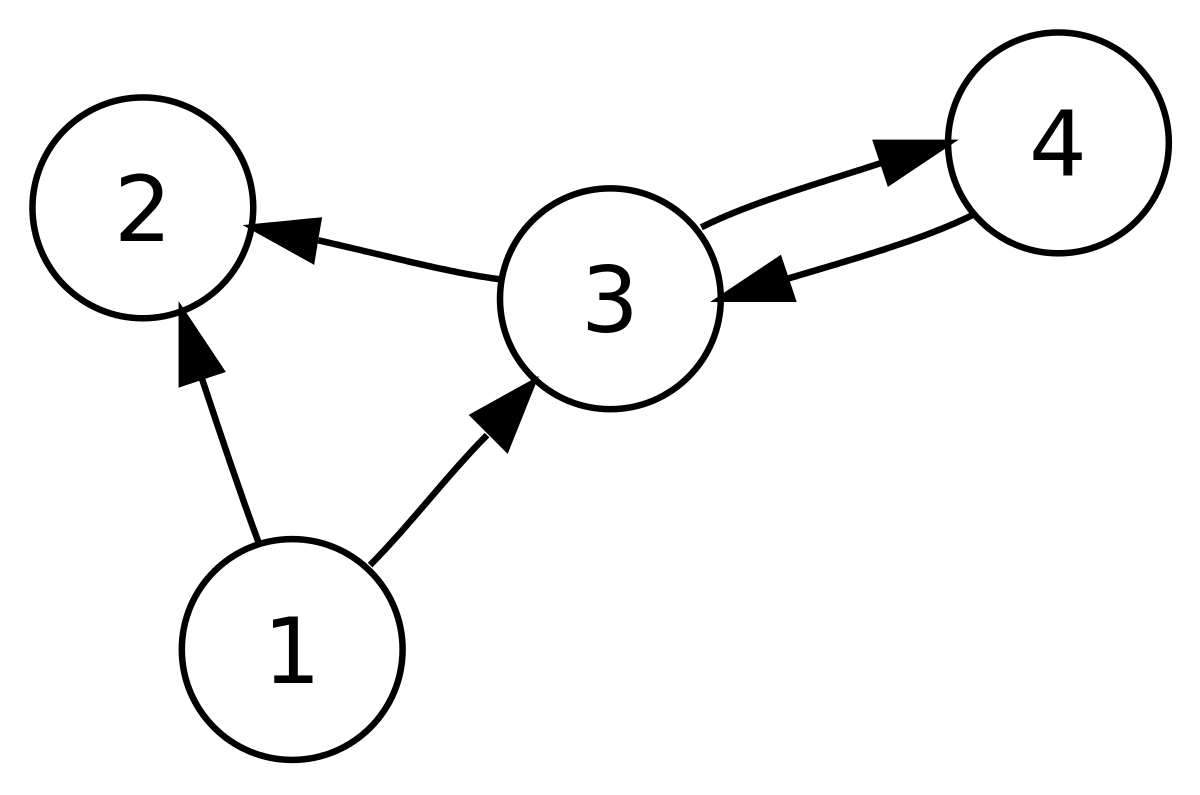
\includegraphics[scale=0.15,center]{./ressources/image/RepDiGraphe.png}
			\caption[Exemple de représentation graphique d'un digraphe.]{Exemple de représentation graphique d'un digraphe.}
			\end{figure}
			
		
		\subsection{Quelques Propriétés:} %%% Arevoire 
			\begin{itemize}[label=$\circ$]
			\item\textbf{Ordre d'un digraphe:}
			est le nombre de sommets n = Card(V) \citep{DUT}.
			
			\item\textbf{taille d'un digraphe:} est le nombre d’arcs m = Card(A) \citep{DUT}.
			
			\item\textbf{Degré dans un digraphe:}
			Le degré d'un sommet $v_{i}$ $\in$ V dans un digraphe G = (V , E) est donnée par la formule :
			\begin{center}
				d($v_{i}$) = $d^+(v_{i}$) + $d^-(v_{i}$\\
			\end{center}			 
			 où $d^+(v_{i}$) est le nombre d'arcs sortants au sommet $v_{i}$ et est appelé degré extérieure et $d^-(v_{i}$) représente le nombre d'arcs incidents et est appelé degré intérieur \citep{muller}.
			 
			 \item\textbf{Voisinage dans un digraphe:}
			 Le voisinage d'un sommet $v_{i}$ $\in$ V, noté V($v_{i}$), dans un digraphe G = (V , E) est:
			 	\begin{center}
				V($v_{i}$) = succ($v_{i}$) $\bigcup$ pred($v_{i}$),
				\end{center}
				
				 avec succ($v_{i}$) qui est l'ensemble des successeurs de $v_{i}$ et pred($v_{i}$) qui l'ensemble de ses prédécesseurs \citep{bac}, i.e le voisinage de $v_{i}$ est l'ensemble des sommets qui lui sont adjacents.
			
			\end{itemize}
			